% Beschreibung der anvisierten Bedienoberfläche (z.B. durch einen Prototyp oder frei gezeichnet) und Erläuterung der Menüstruktur.

\section{Hauptfenster}

\begin{figure}[h]
	\centering
	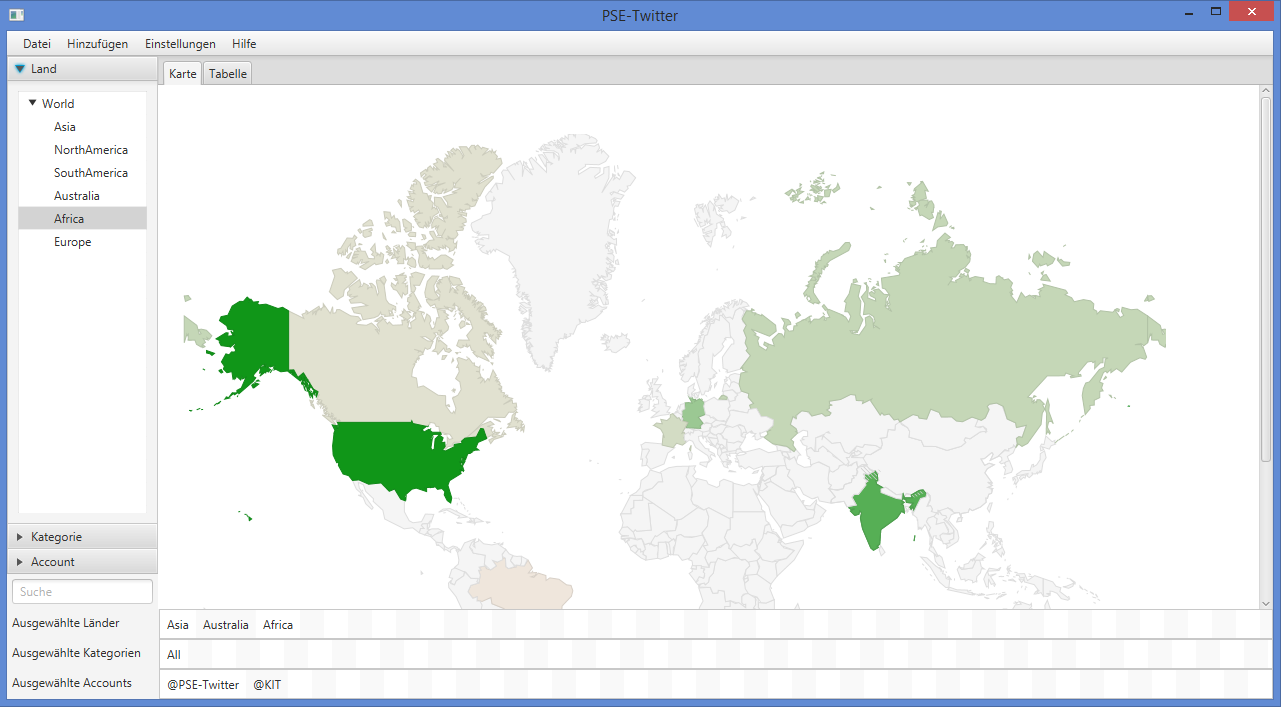
\includegraphics[width=0.9\textwidth]{img/DemoGUIMain.png}
	\caption{Hauptfenster}
	\label{c:Hauptfenster}
\end{figure}

\begin{description}
	\item[Landauswahl] In einer Baumstruktur werden Länder angezeigt. Die Auswahl einzelner Länder erfolgt durch Doppelklick auf das jeweilige Item.
	\item[Kategorienauswahl] Die Kategorien der DMOZ.org Datenbank werden als Baumstruktur angezeigt. Auswahl der Kategorien erfolgt durch Doppelklick auf das jeweilige Item.
	\item[Accountauswahl] In einer Liste werden Accounts angezeigt, die man ebenfalls per Doppelklick auswählen kann.
	\item[Suchfeld] In diesem Textfeld kann ein Begriff eingegeben werden. Je nach geöffnetem Fenster wird nach Land, Kategorie oder Account gesucht.
	\item[Länderübersicht] Eine Liste der bereits ausgewählten Länder.
	\item[Kategorienübersicht] Eine Liste der bereits ausgewählten Kategorien.
	\item[Accountübersicht] Eine Liste der bereits ausgewählten Accounts.
	\item[Karte] Die Weltkarte zeigt zu Beginn nur die Umrisse der Länder. Nach Auswahl von Ländern, Kategorien oder Accounts wird die Karte je nach Verteilung der Retweets zur Auswahl eingefärbt.	
\end{description}

\section{Tabellenansicht}

\begin{figure}[h]
	\centering
	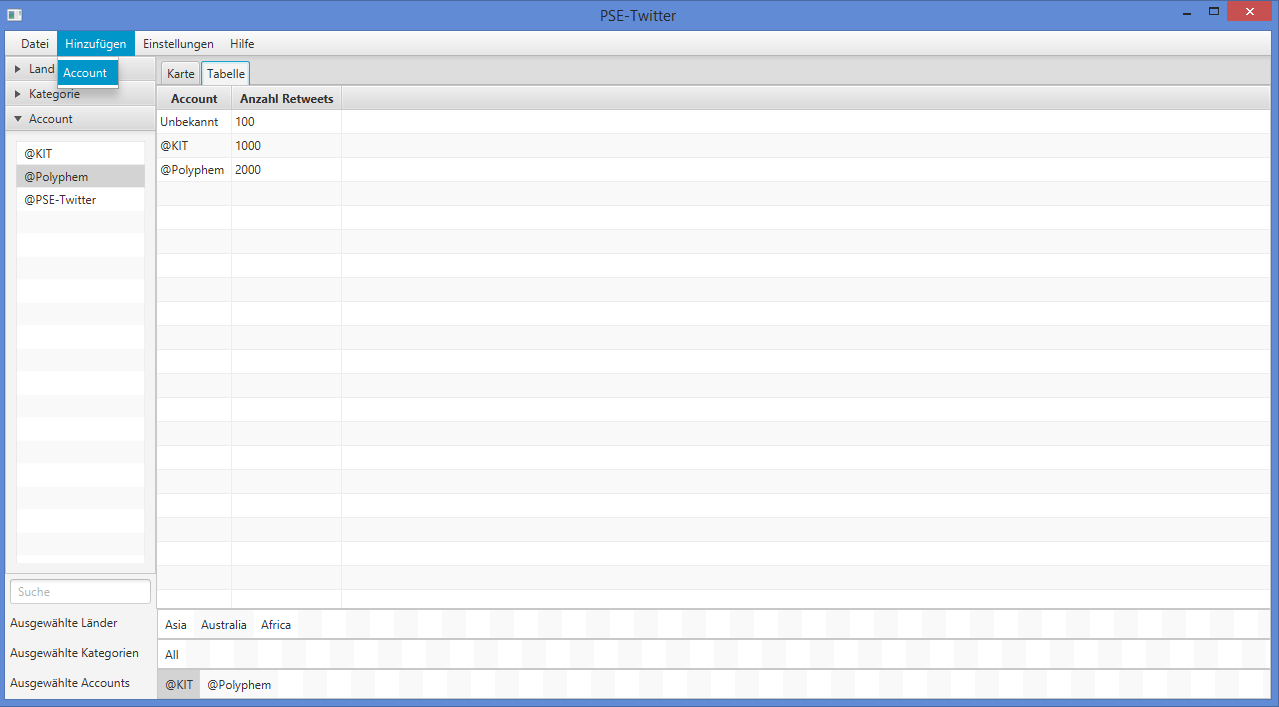
\includegraphics[width=0.9\textwidth]{img/DemoGUITabelleAddAccount.png}
	\caption{Tabellenansicht mit Menu}
	\label{c:Tabellenansicht mit Menu}
\end{figure}

\begin{description}
	\item[Hinzufügen-Menu] Menu-Eintrag, um einen weiteren Account hinzuzufügen. Klicken auf diesen Eintrag öffnet ein Fenster zum Hinzufügen eines Accounts.
	\item[Tabelle] Die Tabelle zeigt Informationen zu den einzelnen ausgewählten, zu Kategorien oder zu Ländern gehörenden Accounts.
\end{description}

\section{Fenster zum Hinzufügen von Accounts}

\begin{figure}[h]
	\centering
	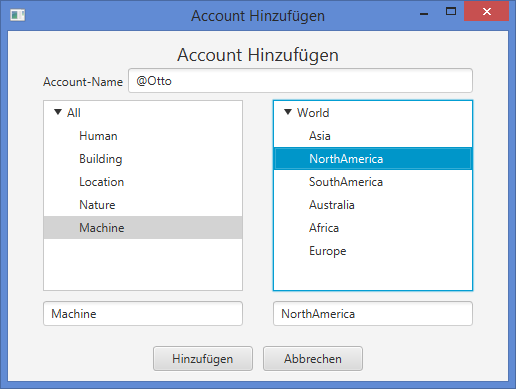
\includegraphics[width=0.9\textwidth]{img/DemoGUIAddAccount.png}
	\caption{Fenster zum Hinzufügen von Accounts}
	\label{c:Fenster zum Hinzufügen von Accounts}
\end{figure}

\begin{description}
	\item[Namensfeld] Textfeld zur Eingabe des Namens des hinzuzufügenden Accounts.
	\item[Hinzufügen-Button] Durch Drücken wird der eingegebene Account überprüft und gespeichert, sowie das Fenster geschlossen.
	\item[Abbrechen-Button] Dadurch wird der Hinzufügen-Vorgang unterbrochen und das Fenster geschlossen.
\end{description}
